\chapter{Revisão Bibliográfica}
\label{chap2}

\section{Manufatura Aditiva}

A Manufatura Aditiva (MA) é um processo de fabricação totalmente customizado, através da impressão em três dimensões de uma peça cuja geometria foi projetada em algum software de modelagem CAD (\textit{Computer-Aided Design}). Diferente da Manufatura Subtrativa, onde retira-se parte do material para se chegar na peça, na MA acontece a sobreposição de camadas deste material, que são unidas através de diferentes processos \cite{gibson2021additive}. A tecnologia começou sendo utilizada para fabricação de peças poliméricos e cerâmicos, sendo depois expandida para outros materiais como ligas metálicas para peças para a indústria, que se interessou pelas vantagens de redução de custos e tempo de fabricação, bem como a possibilidade de fabricar peças com geometrias complexas. A fabricação em MA consiste, basicamente, na deposição gradual de um material camada a camada \cite{srinivas2017critical}. Este material é aquecido através de um sistema de aquecimento e depositado por algum sistema robótico cuja trajetória é computadorizada, os chamados sistemas CNC (Controle Numérico Computadorizado). O fluxo da fabricação via MA é ilustrado na figura \ref{fig:ma_steps}:
\newpage
\begin{figure}[hbt!]
    \centering
    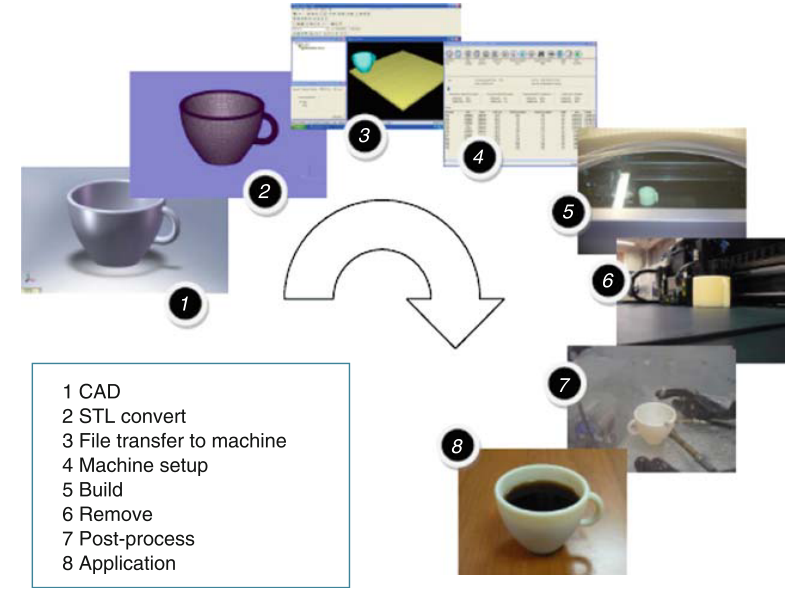
\includegraphics[width=0.8\linewidth]{Imagens/chap02/ma_steps.png}
    \caption{Etapas do processo de MA \cite{gibson2021additive}.}
    \label{fig:ma_steps}
\end{figure}
\begin{enumerate}[start=0]
    \item Seleção da técnica e material: Dependendo da aplicação, uma técnica e material correspondentes são mais recomendados. A técnica e o material influenciarâo nas demais etapas (ex: peças fabricadas por SLM não podem possuir regiões vazias totalmente internas, pois o pó não teria por onde escapar.

    \item Modelagem em CAD: Esta etapa consiste na modelagem de uma geometria tridimensional que compreende totalmente a superfície externa de um objeto.

    \item Conversão para arquivo STL: O arquivo STL contém toda a informação a respeito da superfície geométrica criada em CAD.

    \item Transferência do arquivo para a máquina de MA (Fatiamento): O arquivo necessita ser transferido para máquina para que ela o manipule, ajeitando posicionamento, tamanho e direcionamento.

    \item Configuração da máquina: Antes da fabricação, é necessário configurar alguns parâmetros para otimizar o resultado, tais como  a espessura da camada, a fonte de energia e o tempo de fabricação.
    
    \item Fabricação: Esta etapa é gerenciada automaticamente pela máquina. Só é necessário um monitoramento superficial para assegurar de que ainda há material, se a impressão está indo bem, etc.

    \item Remoção: Após a fabricação, é necessário remover a peça da máquina. Algumas máquinas possuem mecanismos de segurança que impedem a sua abertura até que a temperatura esfrie até um determinado valor.

    \item Pós-processamento: Algumas peças necessitam de acabamento, como limpeza e remoção de suportes de impressão ou tratamento térmico.

    \item Aplicação: Depois de todos esses processos, a peça está pronta para ser aplicada.
\end{enumerate}

As empresas que utilizam a MA possuem diferencial competitiva ao possuírem reduzidos custos e tempo de fabricação, maior facilidade em atender restrições ambientais, flexibilidade no projeto das peças, entre outros fatores \cite{srinivas2017critical}.

\subsection{Manufatura Aditiva a Arco e Arame (WAAM)}
Recentemente, as grandes fabricantes de peças de \textit{design} complexo começaram a ver na WAAM uma oportunidade de produzir peças com melhor qualidade e a menor custo, sem a necessidade de ferramentas específicas, beneficiando a indústria ao permitir uma manufatura decentralizável, rápida e facilmente adaptável, o que é de suma importância no contexto da Indústria 4.0. O processo de WAAM consiste na fusão de um arame usado como material de deposição por um arco elétrico, e por isso entra na classe dos processos de deposição por energia direta (DED) \cite{vafadar2021advances}. Em comparação com outros processos de MA, WAAM tem taxas de resfriamento inferior e uma quantidade de calor utilizada superior, o que é benéfico para a maioria dos materiais disponívies no mercado \cite{treutler2021current}. Devido a extensa e consolidada pesquisa realizada em soldagem a arco para superfícies e juntas, o conhecimento a cerca do comportamento dos materiais e processos foi transferido para WAAM, agilizando o desenvolvimento da técnica \cite{oliveira2020revisiting}.A figura \ref{fig:waam_papers} mostra o número de publicações na área, por ano, ilustrando o crescimento do interesse por essa tecnologia e ratificando a importância do tema.
\newpage
\begin{figure}[hbt!]
    \centering
    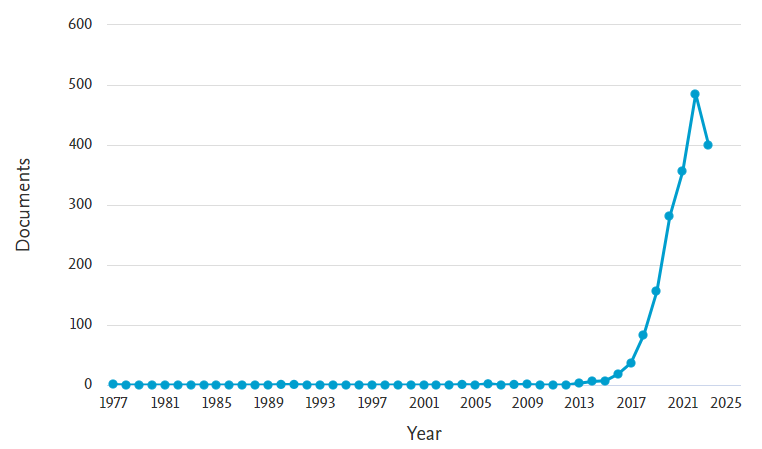
\includegraphics[width=0.8\linewidth]{Imagens/chap02/waam_papers.png}
    \caption{Contribuições de artigos publicados em jornais técnicos envolvendo WAAM. Fonte: SCOPUS.}
    \label{fig:waam_papers}
\end{figure}

Graças a grande quantidade de calor utilizada no processo, é comum que as peças produzidas sofram deformações e acumulem tensões residuais, levando ao risco de falhas. Além disso, baixa precisão geométrica e acabamento ruim são outros problemas causados pelo empilhamento de camadas de cordões \cite{ding2015wire}. A figura \ref{fig:waam_parts} mostra exemplos de peças produzidas por WAAM.

\begin{figure}[hbt!]
    \centering
    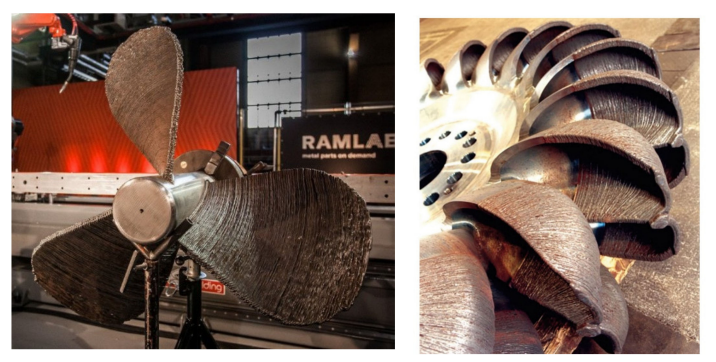
\includegraphics[width=0.8\linewidth]{Imagens/chap02/waam_parts.png}
    \caption{Hélice (esquerda) e tubina hídrica (direita) fabricados por WAAM \cite{feldmann20193d}.}
    \label{fig:waam_parts}
\end{figure}

\newpage
\subsection{Diferentes processos dentro da WAAM}
O processo de WAAM funciona através do depósito, camada a camada, do material metálico fundido pelo arco elétrico, que pode possuir diferentes fontes de energia. Os mais comuns são soldagem de arco de metal a gás (GMAW), soldagem de arco de metal Tungstênio a gás (GTAW) e soldagem a arco de plasma (PAW). \cite{pan2018arc}

\subsubsection{GMAW}
GMAW é um processo de soldagem no qual um arco elétrico se forma entre um eletrodo de arame metálico (que se consome no processo) e a base de trabalho. O arame geralmente está perpendicular ao plano da base. Existem diferentes métodos de extrusão do arame dentro do processo de GMAW, como por exemplo pulso-spray, spray ou transferência de metal a frio (CMT), uma variante do padrão de GMAW onde o arame é retraído e extrudado periodicamente com o intuito de controlar a transferência das gotículas de metal fundido. Esse método é o mais utilizado pela pequena quantidade de calor necessária \cite{pan2018arc}. A figura \ref{fig:gmaw_scheme} ilustra o processo de GMAW.

\begin{figure}[hbt!]
    \centering
    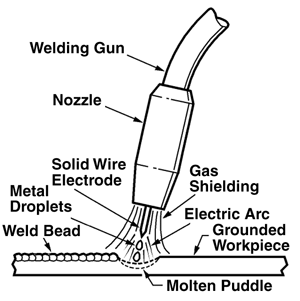
\includegraphics[width=0.6\linewidth]{Imagens/chap02/gmaw_scheme.png}
    \caption{Ilustração do processo de GMAW \cite{azadi2017simultaneous}.}
    \label{fig:gmaw_scheme}
\end{figure}

\subsubsection{GTAW}
No processo de GTAW, um eletrodo de tungstênio, não consumido, é usado para fundir um outro arame metálico, cujo material é depositado, como ilustrado na figura \ref{fig:gtaw_scheme}. Durante o processo de deposição, a orientação da alimentação do arame influencia a qualidade da transferência. Um modelo matemático foi desenvolvido para otimizar a direção e posição da alimentação do arame para melhorar a acurácia da deposição \cite{geng2017optimization}.

\begin{figure}[hbt!]
    \centering
    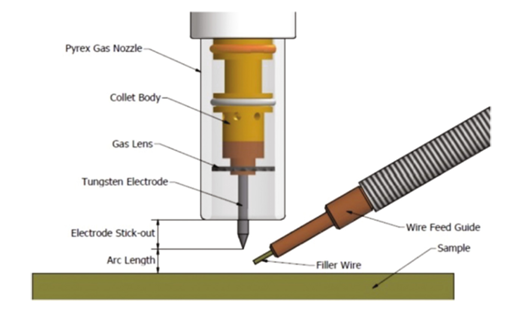
\includegraphics[width=0.8\linewidth]{Imagens/chap02/gtaw_scheme.png}
    \caption{Ilustração do processo de GTAW \cite{hoye2015characterisation}.}
    \label{fig:gtaw_scheme}
\end{figure}

\subsubsection{PAW}
O processo de PAW consiste num arco de plasma cuja densidade energética pode chegar a 3 vezes maior que o mesmo via GTAW, causando menos distorção nas soldas e menores pontos de solda, bem como maiores velocidades de soldagem, como ilustrado na figura \ref{fig:paw_scheme}. 

\begin{figure}[hbt!]
    \centering
    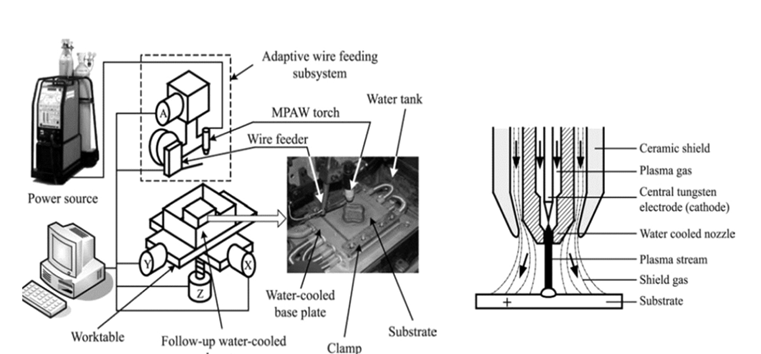
\includegraphics[width=0.7\linewidth]{Imagens/chap02/paw_scheme.png}
    \caption{Ilustração do processo de PAW e detalhes do arco de plasma \cite{aiyiti2006investigation}.}
    \label{fig:paw_scheme}
\end{figure}

\newpage
A figura \ref{fig:waam_steps} mostra as etapas da produção de uma peça via WAAM. São elas:
\begin{enumerate}[label=(\textit{\roman*})]
    \item Projeto da peça em software CAD, e adaptações necessárias para conformar-se ao processo de WAAM.
    \item  Definição da altura da camada e fatiamento em software dedicado.
    \item Definir a trajetória do maçarico, controlado por um manipulador robótico.
    \item Especificar a geometria do cordão durante a impressão.
    \item Definir os parâmetros de deposição indireta (IDP) para alcançar as características desejadas.
    \item Configurar os parâmetros de deposição na fonte de energia e mandar a trajetória para o robô. 
    \item Construir a peça. 
    \item Executar o pós-processamento da peça, atingindo o acabamento ou acurácia geométrica desejados.
\end{enumerate}

\begin{figure}[hbt!]
    \centering
    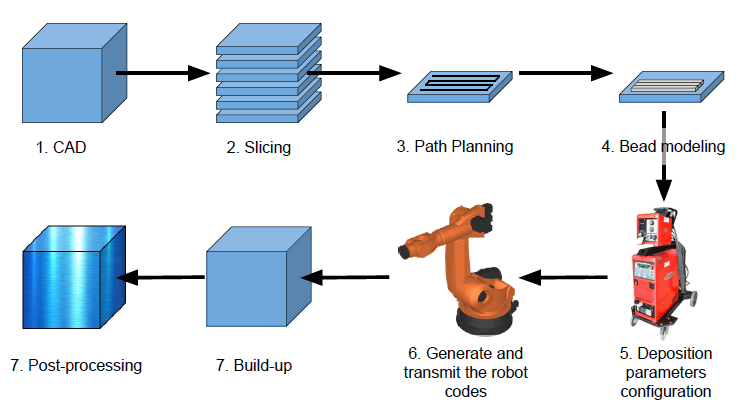
\includegraphics[width=0.8\linewidth]{Imagens/chap02/waam_steps.png}
    \caption{Etapas do processo de WAAM \cite{ding2016bead}.}
    \label{fig:waam_steps}
\end{figure}

\subsection{Defeitos comuns na WAAM}
Para que os sistemas de WAAM sejam amplamente utilizados na indústria, é necessário investigar e mitigar os defeitos de fabricação dessa tecnologia. Porosidade, deformação, tensão residual e craqueamento são alguns desss defeitos, que precisam ser evitados a fim de que as peças possam ser utilizadas em sua plena capacidade. Esses defeitos podem acontecer por conta de trajetórias não otimizadas durante a fabricação, configuração errada dos parâmetros de deposição, deformação associada ao acúmulo de calor, arames de baixa qualidade, contaminação, etc \cite{wu2018review}. A figura \ref{fig:waam_defects} descreve as correlações entre possíveis defeitos na fabricação via WAAM utilizando aço. 

\begin{figure}[hbt!]
    \centering
    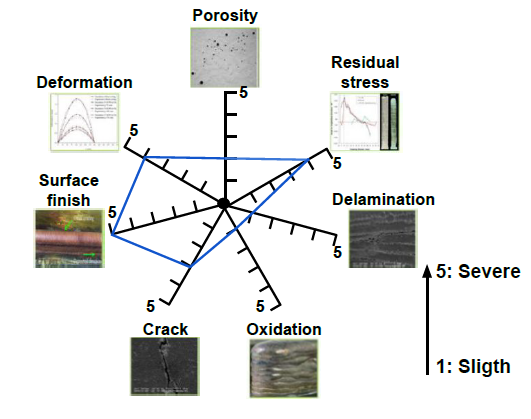
\includegraphics[width=0.8\linewidth]{Imagens/chap02/waam_defects.png}
    \caption{Correlação entre defeitos de fabricação via WAAM utilizando aço. Adaptado de \cite{wu2018review}.}
    \label{fig:waam_defects}
\end{figure}

\subsubsection{Tensão residual}
A tensão residual é o principal agente causador das distorções, que podem levar a falhas mecânicas. Ela consiste nas tensões internas que permanecem após todas as forças internas serem removidas, e é causada principalmente pela expansão e encolhimento causado pelo rápido aquecimento e esfriamento da peça. É impossível eliminá-la completamente, visto que o processo de WAAM depende de grandes quantidades de calor, no entanto, é possível mitigá-la com o tratamento térmico após a fabricação \cite{wu2018review}. 

\subsubsection{Porosidade}
Outro defeito comum presente no processo de WAAM é a presença de poros nas peças. Essa porosidade é causada por diversos fatores, como contaminação do arame, acúmulo de gases na peça, trajetórias não otimizadas, etc. Para reduzir este defeito, é necessário evitar os problemas descritos acima \cite{wu2018review}. 

\subsubsection{Delaminação}
A delaminação consiste na separação das camadas de impressão via WAAM. Ela acontece principalmente quando não há a fusão completa das camadas adjacentes, podendo ser visível por inspeção visual. Pré aquecer o substrato pode previnir este defeito \cite{wu2018review}.

\subsection{Parâmetros diretos e indiretos de deposição}
Os parâmetros de deposição podem ser divididos entre diretos (DDP) e indiretos (IDP) \cite{ozcelik2003modeling}. Os DDP são os parâmeteos de "saída", e estão relacionados com as características do material depositado, como geometria do cordão, propriedades mecânicas, etc. Já os IDP são os parâmetros de "entrada", e são as configurações utilizadas para se alcançar uma determinada característica desejada, como corrente (I), tensão (V), velocidade de viagem (TS), velocidade de alimentação do arame (WFS), entre outros. A figura \ref{fig:waam_params} descreve ambos os grupos de parâmetros. 

\begin{figure}[hbt!]
    \centering
    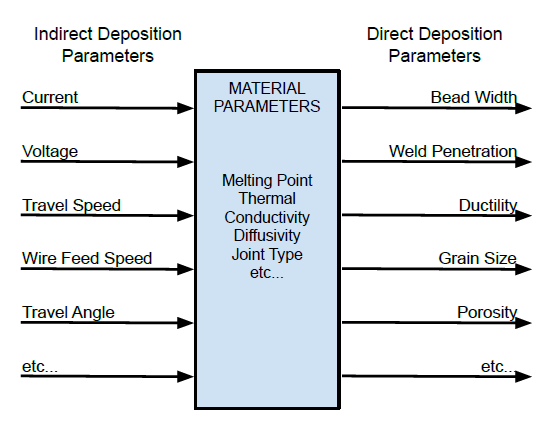
\includegraphics[width=0.8\linewidth]{Imagens/chap02/waam_params.png}
    \caption{Parâmetros de entrada e saída. \cite{ozcelik2003modeling}.}
    \label{fig:waam_params}
\end{figure}

\subsubsection{Corrente}
A corrente é um IDP elétrico intrínseco a fonte utilizada na soldagem via WAAM. Mantendo todos os outos parâmetros fixos, a corrente (I) influencia diretamente a velocidade de alimentação do arame (WFS) modelada na equação \ref{eq:current_wfs}

\begin{equation}
WFS = aI + bl_{so}I^2
\label{eq:current_wfs}
\end{equation}

onde $a$ é a constante de proporcionalidade para o aquecimento do anodo/catodo, cuja magnitude depende da polaridade, composição e outros fatores; $b$ é outra constante de proporcionalidade relacionada a resistência térmica, e $l_{so}$ é a extensão máxima (\textit{stick-out}) do eletrodo. Além disso, o aumento da corrente resulta em:

\begin{enumerate}
    \item Maior taxa de deposição (DR).
    \item Maior profundidade e largura de penetração do cordão.
    \item Maior largura e altura do cordão.
\end{enumerate}

\subsubsection{Tensão}
A tensão é um IDP importante no processo de GMAW, influenciando na própria corrente mencionada acima, no comprimento do arco, e outros IDPs.

\subsubsection{Velocidade de viagem do maçarico}
A velocidade de viagem (TS) é um parâmetro de deposição que depende da trajetória do robô, determinada pelo processo de deposição. A TS é simplesmente o módulo da velocidade linear tangente a curva da trajetória do robô, como mostrado na equação \ref{eq:ts_eq}. 

\begin{equation}
TS = \sqrt{V_x^2 + V_y^2}
\label{eq:ts_eq}
\end{equation}

A TS influencia as características do cordão e por isso é um importante IDP, sendo desejado que seja mantida constante durante a impressão para evitar variações na geometria do cordão. A TS também influencia outros DDPs, por exemplo, na penetração e largura do cordão. Quanto maior for a TS, menor são esses parâmetros mencionados \cite{ozcelik2003modeling}.

\subsubsection{Velocidade de alimentação do arame}
A velocidade de alimentação do arame (WFS) consiste na velocidade em que o arame é extrudado do local onde está armazenado em direção ao maçarico, onde será fundido e depositado. A WFS influencia positivamente a altura do cordão soldado. \cite{srivastava2023wire}.

% Além da TS, a distância entre o tubo e a base de trabalho e o fluxo de gás de proteção são alguns dos IDP definidos na etapa de planejamento e executadas durante a deposição. Em GMAW o gás de proteção serve para canalizar o arco elétrico. 

A figura \ref{fig:gmaw_idp_ddp} descrevem os IDP e DDP dentro do processo de GMAW.
\begin{figure}[hbt!]
    \centering
    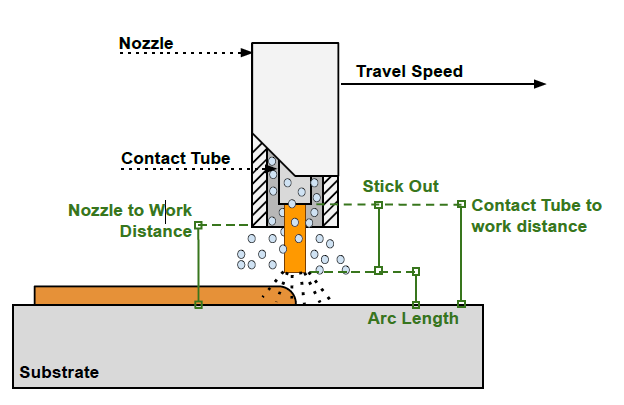
\includegraphics[width=0.46\linewidth]{Imagens/chap02/gmaw_idp.png}
    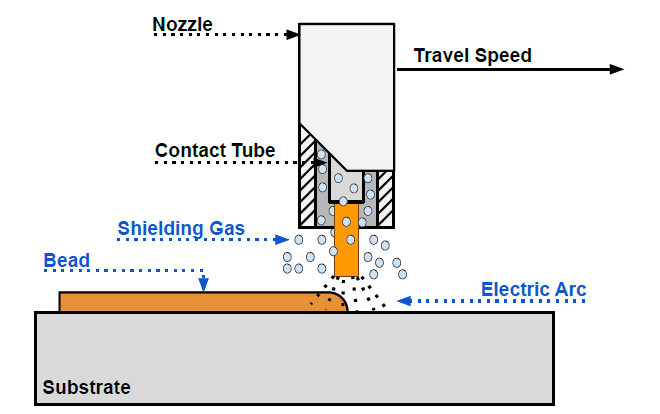
\includegraphics[width=0.46\linewidth]{Imagens/chap02/gmaw_ddp.png}
    \caption{Alguns IDPs (esquerda) en DDPs (direita) do processo de GMAW \cite{ozcelik2003modeling}.}
    \label{fig:gmaw_idp_ddp}
\end{figure}

% \begin{figure}[hbt!]
%     \centering
%     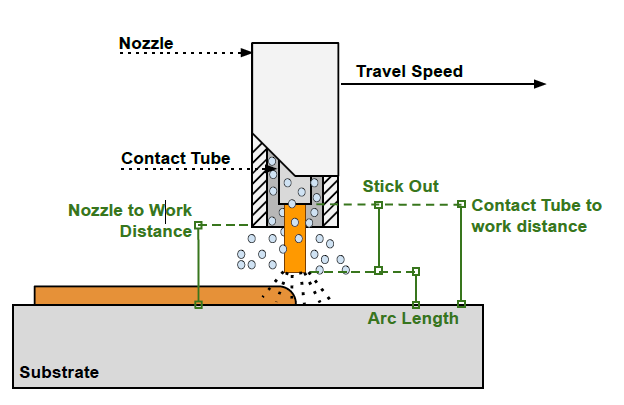
\includegraphics[width=0.8\linewidth]{Imagens/chap02/gmaw_idp.png}
%     \caption{TS e outros IDPs do processo GMAW \cite{ozcelik2003modeling}.}
%     \label{fig:gmaw_idp}
% \end{figure}

% \begin{figure}[hbt!]
%     \centering
%     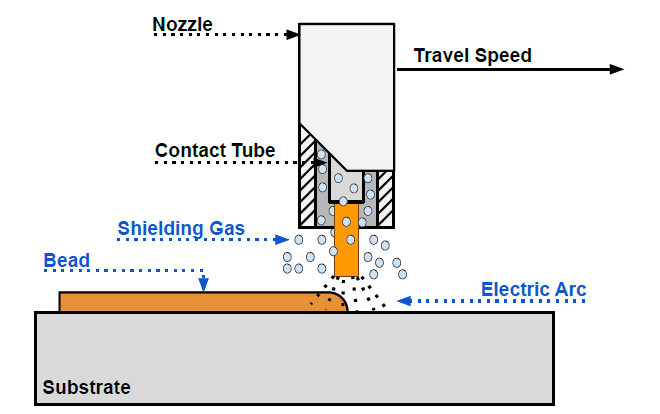
\includegraphics[width=0.8\linewidth]{Imagens/chap02/gmaw_ddp.png}
%     \caption{Visão lateral do maçarico no processo GMAW e alguns DDPs \cite{ozcelik2003modeling}.}
%     \label{fig:gmaw_ddp}
% \end{figure}

\newpage
\subsection{Geometria do cordão simples}
Como descrito anteriormente, é de suma importância entender as relações entre os parâmetros de deposição e a geometria do cordão simples. Alguns métodos matemáticos foram desenvolvidos para representar o perfil geométrico do cordão, correlacionando-o com os parâmetros de entrada (alguns mais simples, como parábolas, arcos circulares, e outros mais complexos, funções logísticas ou gaussianas). De forma geral, o principal parâmetro que influencia na geometria do cordão é a velocidade de alimentação do arame (WFS) e a velocidade de viagem (TS) \cite{cao2011overlapping}. 

Possuir um modelo geométrico robusto é de suma importância para o desenvolvimento de um sistema de MA inteligente e moderno, já que pode ser utilizado em uma malha de controle realimentado, aumentando a qualidade do acabamento das peças fabricadas via WAAM. 

Neste trabalho será utilizado apenas modelos de cordão simples no processo de GMAW. A próxima seção aborda toda a modelagem do simulador utilizado para gerar os dados que alimentam a rede.

\section{Simulação geométrica em GMAW}
\label{sec:simulation}
Diversos modelos estáticos de equações de transferência de massa e energia foram desenvolvidos ao longo dos anos para analisar as dinâmicas do processo de WAAM. Neste trabalho, será utilizado uma simulação para um modelo de cordão simples impresso em GMAW como fonte de geração de dados para o treinamento da rede. 

A modelagem em questão relaciona os parâmetros de entrada $f$ (WFS), $I_r$ (corrente), $l_c$ (Distância entre a ponta do arame e a base - CTWD) e $v$ (TS), e os parâmetros de saída $w$ (largura) e $h$ (altura) do cordão único. Essa modelagem acontece em duas etapas: a primeira consiste no processo GMAW, que relaciona os quatro parâmetros de entrada aos parâmetros $Q$ (potência líquida) e $A_c$ (área de seção reta), e a segunda consiste num modelo geométrico estático que relaciona esses dois parâmetros com a largura e altura do cordão, como ilustra a figura \ref{fig:sim_blocks}

\begin{figure}[hbt!]
    \centering
    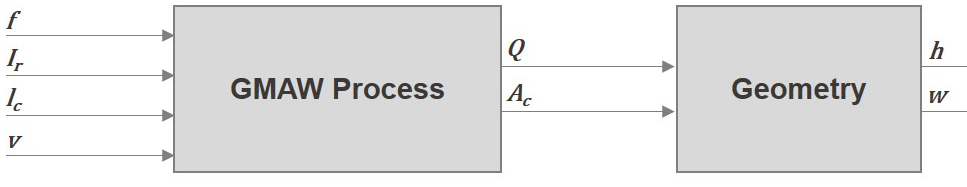
\includegraphics[width=0.8\linewidth]{Imagens/chap02/sim_blocks.png}
    \caption{Diagrama de blocos da modelagem utilizada \cite{bendia2021multivariable}.}
    \label{fig:sim_blocks}
\end{figure}

\subsubsection{Modelo do processo GMAW}
O modelo do processo GMAW consiste num modelo não linear de 5ª ordem (figura \ref{fig:gmaw_model}) considerando a dinâmica elétrica da fonte e a dinâmica térmica da deposição da gotícula metálica do cordão. 

\begin{figure}[hbt!]
    \centering
    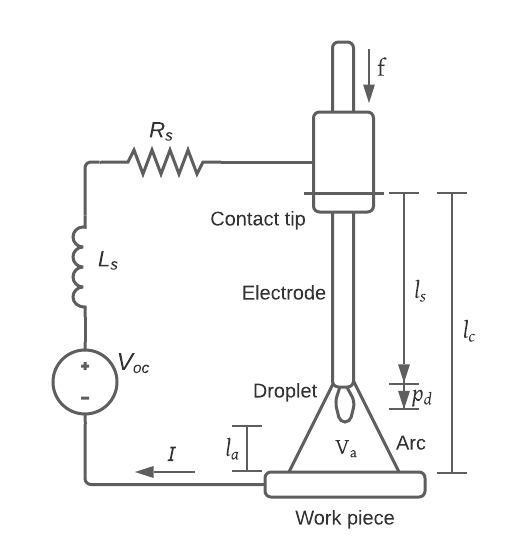
\includegraphics[width=0.5\linewidth]{Imagens/chap02/gmaw_model.png}
    \caption{Modelo termoelétrico do processo GMAW \cite{bendia2021multivariable}.}
    \label{fig:gmaw_model}
\end{figure}

A dinâmica elétrica da fonte que modela a transferência de energia é dada pela equação:

\begin{equation}
    \frac{dI}{dt} = \frac{1}{L_s} [V_{oc} - (R_a+R_s+R_L)I - V_0 -E_a(l_c-l_s)]
\end{equation}

onde $L_s$ é a indutância da fonte, $V_{oc}$ é a tensão de circuito aberto da fonte, $R_s$ é a resistência da fonte, $R_a$ é a resistência do arco, $R_L$ é an resistência do eletrodo, $V_0$ é a constante da zona de carga, $E_a$ é o fator de comprimento do arco e $l_s$ é a extensão do arame.  A resistência do eletrodo $R_L$ é função do comprimento: 
\begin{equation}
    R_L = \rho[l_s + 0.5(r_d+p_d)]
\end{equation}
onde $\rho$ é a resistividade do eletrodo, $r_d$ é o raio da gotícula e $p_d$ é a distância entre o centro de massa da gotícula e o eletrodo \cite{bendia2021multivariable}. Considerando uma fonte onde a corrente de deposição $I$ é mantida controlada numa corrente de referência $I_r$, $V_{oc}$ é usada como uma variável de controle definida por: 

\begin{equation}
    V_{oc} = K_v(I_r-I) + \bar{V}_{oc}
\end{equation}

onde $\bar{V}_{oc}$ é o ponto de opperação da tensão de circuito aberto e $K_v$ é um ganho proporcional. Portanto, a dinâmica da corrente em malha fechada é:

\begin{equation}
    \frac{dI}{dt} = \frac{1}{L_s} [K_vI_r - (R_a+R_s+\rho l_S + K_v)I + \bar{V}_{oc} - V_0 -E_a(l_c-l_s)]
\end{equation}

A tensão $V_a$ e potência $P_a$ do arco são:
\begin{align}
    V_a = V_0 + R_aI + E_a(l_c-l_s) \\
    P_a =  R_aI^2 + [E_a(l_c-l_s) + V_0]I
\end{align}

Finalmente, a taxa de transferência de energia do arco para a base é modelada pela eficiência $\eta$, e a potência líquida $Q$ é:
\begin{equation}
    Q = \eta P_a
\end{equation}

A equação de balanço de massa é definida como a diferença entre o material entrando no sistema, que depende da WFS $f$, e o material saindo o sistema, através da deposição da solda. Assumindo que a densidade do eletrodo $\rho_w$ é constante, o fluxo de material que entra é definido como $A_w f$, onde $A_w$ é a área de seção reta do arame. Já o fluxo de material que sai é definido como $M_r$. Com isso, a dinâmica do balanço de massa é:
\begin{align}
    A_w\frac{dl_s}{dt} &= Aw f - M_r \\
    M_r &= C_2\rho l_s I^2 + C_1 I
\end{align}
onde $C_1$ e $C_2$ são constantes de fusão.

Da perspectiva de um sistema de coordenadas movendo-se junto com o maçarico com velocidade $v$, como mostrado na figura \ref{fig:torch_coords}, o fluxo volumétrico de deposição do cordão é definido como $\frac{dV}{dt} = A_c v$. O volume depositado é igual ao fluxo de saída do material $M_r$. Portanto, $M_r = A_c v$:
\begin{equation}
    A_c = \frac{C_2\rho l_s I^2 + C_1 I}{v}
\end{equation}

\begin{figure}[hbt!]
    \centering
    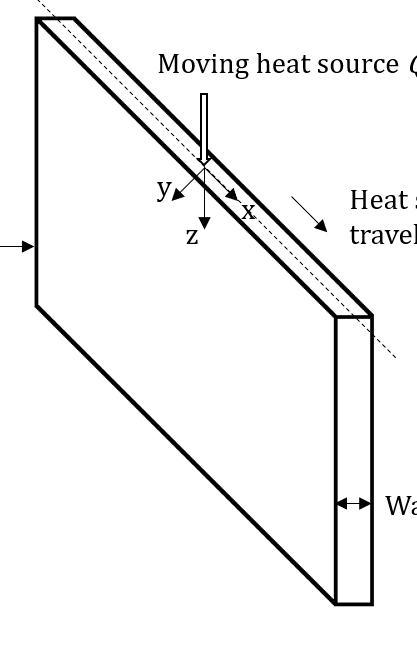
\includegraphics[width=0.2\linewidth]{Imagens/chap02/torch_coords.png}
    \caption{Sistemas de coordenadas do maçarico \cite{bendia2021multivariable}.}
    \label{fig:torch_coords}
\end{figure}

Com isso, a dinâmica do processo é definida pelo sistema não linear \cite{bendia2021multivariable}:
\begin{align}
    \frac{dl_s}{dt} &=-\frac{1}{A_w}(C_2\rho l_s I^2 + C_1 I) + f \\
    \frac{dI}{dt} &= \frac{1}{L_s} [K_vI_r - (R_a+R_s+\rho l_S + K_v)I + \Delta V_0 -E_a(l_c-l_s)]
\end{align}

onde $\Delta V_0 = \bar{V}_{oc} - V_0$. As variáveis de estado são $l_s (m)$ e $I (A)$, os parâmetros de entrada são $f (m/s)$ e $I_r (A)$, e os de saída são $Q (W)$ e $A_c (m^2)$. 

\subsubsection{Modelo geométrico}
As dimensões do cordão podem ser calculadas do campo de temperaturas no substrato no entorno de uma fonte de calor em movimento (o maçarico). A curva isotérmica correspondente a temperatura de fusão dá a forma da piscina de fusão. Considerando uma parede fina de substrato como mostrado na figura \ref{fig:torch_coords}, a solução de Rosenthal é:

\begin{equation}
    T - T_0 = \frac{Q}{2\pi k w_t}K_0\left(\frac{r_{xz}v}{2\alpha}\right)\exp{\frac{-xv}{2\alpha}} \label{eq:rosenthal}
\end{equation}

onde $T$ é a temperatura de um ponto nas coordenadas $(x,z)$ em relação ao maçarico, $T_0$ é a temperatura do substrato na saída do maçarico, $k$ é a condutividade térmica, $\alpha$ é a difusividade térmica, $w_t$ é a espessura da parede, $v$ é a TS, $r_{xz} = \sqrt{x^2+z^2}$ é a distância euclidiana do ponto ao maçarico e $K_0$ é a função de Bessel modificada de ordem zero do segundo tipo. Em \cite{rios2018analytical} uma extensão de \ref{eq:rosenthal} é proposta para calcular a potência desejada a fim de alcançar uma determinada dimensão geométrica:

\begin{equation} 
    Q = 4kw_e(T_m-T_0)(0.2+\frac{v}{2\alpha}d_a) \label{eq:rios}
\end{equation}

onde $T_m$ é a temperatura de fusão, $w_e$ é a largura efetiva do cordão e $d_a$ é a profundidade aparente do cordão. As características geométricas do cordão estão ilustradas na figura \ref{fig:bead_geom} e são calculadas por:
\begin{align}
    w &= 2r \label{eq:w}\\
    w_e &= 2ra\cos(\theta/2) \\
    h &= 2r\sin(\theta/2) \\
    d_a &= \frac{w+h}{2} \label{eq:d_a} \\
\end{align}

\begin{figure}[hbt!]
    \centering
    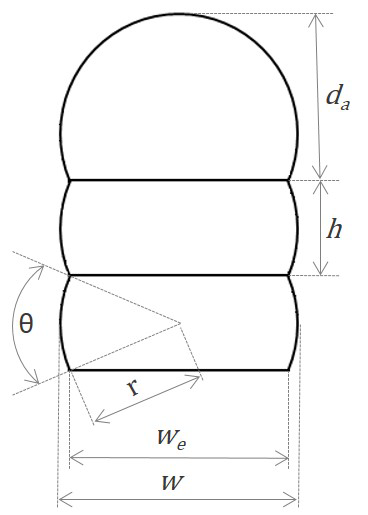
\includegraphics[width=0.3\linewidth]{Imagens/chap02/bead_geom.png}
    \caption{Parâmetros geométricos do cordão \cite{bendia2021multivariable}.}
    \label{fig:bead_geom}
\end{figure}

A área da camada única do cordão $A_c$ é dada por:
\begin{equation}
    A_c = 0.5(w^2\arctan(h/w_e) + w_eh)
\end{equation}
Para  $h < \frac{w_e}{2} < \frac{w}{2}$, então $\frac{h}{w_e} < \frac{1}{2}$ e $\arctan(h/w_e) \approx h / w_e$, então:
\begin{equation}
    A_c = \frac{1}{2} \left(w^2\frac{h}{w_e} + w_e h\right) \label{eq:area_bead}
\end{equation}
Considerando a área útil dada pelo produto $w_e h$ então a eficiência de deposição é:
\begin{equation}
    \eta_d = \frac{w_e h}{A_c} \label{eq:eta_d}
\end{equation}

Substituindo \ref{eq:area_bead} in \ref{eq:eta_d} para achar a relação entre $w$ e $w_e$:
\begin{equation}
    w = \sqrt{\frac{2-\eta_d}{\eta_d}}w_e
\end{equation}

Com isso, considerando as equações \ref{eq:w}-\ref{eq:d_a} e \ref{eq:area_bead} em \ref{eq:rios}, $w_e$ pode ser expresso em função de $Q$, $v$ e $A_c$:
\begin{equation}
    \sqrt{(2-\eta_d)/eta_d}w_e^2 + 0.8\frac{\alpha}{v}w_e + \eta_dA_c - \frac{Q\alpha}{k\Delta T v} = 0
\end{equation}

onde $\Delta T = T_m - T_0$. Esse polinômio do segundo grau tem raízes se $p = \left(\eta_d-\frac{Q\alpha}{k\Delta T v}\right)/\sqrt{\frac{2-\eta_d}{\eta_d}}$ for negativo. Essa condição é satisfeita se:
\begin{equation}
    Q > \frac{k\Delta T v}{\alpha} \eta_d A_c \label{eq:q_cond}
\end{equation}
 
Portanto, se \ref{eq:q_cond} for satisfeita, $w_e$ e $h$ são dados por:
\begin{align}
    w_e &= -\frac{0.4\alpha}{k_w v} + \sqrt{\left(\frac{0.4\alpha}{k_wv}\right)^2 - \frac{1}{k_w}\left(\frac{2A_c}{k_w^2+1} - \frac{Q\alpha}{k\Delta T v}\right)} \\
    h &= \eta_d \frac{A_c}{w_e}
\end{align}

onde $k_w = \sqrt{(2-\eta_d)/\eta_d}$.

% \subsubsection{Linearização do modelo}

\section{\textit{Machine Learning}}
\textit{Machine Learning} (ML), ou aprendizado de máquinas, são algoritmos e processos em que a máquina não sabe a resposta para determinada tarefa. No caso deste projeto, focamos nos algoritmos de ML para análise de dados. Esses algoritmos podem ser de aprendizado supervisionado ou não-supervisionado. Porém, tão importante quanto saber qual o melhor algoritmo utilizar, é saber quais dados utilizar, bem como processá-los \cite{alpaydin2020introduction}. A base de treinamento dos modelos de ML são os dados. É de suma importância possuir dados de qualidade, que tenham riqueza da informação que é necessária para aquele determinado problema. 

\subsection{Métodos de aprendizado}
O aprendizado de todos os modelos e algoritmos de ML pertencem a um desses três grupos: Aprendizado Supervisionado, Não supervisionado, ou por reforço.  No caso do aprendizado supervisionado, os dados de entrada $X$ e saída $Y$ são conhecidos. Com isso, a tarefa consiste em utilizar $X$ para produzir uma estimativa $\hat{Y}$ que é comparada a $Y$. No aprendizado não supervisionado, os dados de saída $Y$ não são conhecidos, e a tarefa é estimar os valores de saída de cada ponto de $X$ de forma que pontos distintos possuem valores de $y$ distintos, e pontos próximos possuem valores de $y$ próximos. Por último, os algoritmos de aprendizado por reforço funcionam com a recompensa positiva ou negativa de determinadas ações, que são usadas para treinar uma política que consegue escolher aquela ação que maximiza a recompensa. 

\subsection{\textit{Deep Learning}}
A área do \textit{Deep Learning} (DL) consiste na modelagem das redes neurais artificiais (ANN), que se inspiram no cérebro humano. A primeira e mais básica dela é o Perceptron Multicamadas (MLP), que utiliza uma rede de neurônios interconectados que realizam operações matemáticas a fim de mapear, via aprendizado supervisionado, dados de entrada $X$ e de saída $Y$. 

\subsubsection{MLP}
O neurônio funciona recebendo um vetor de valores de entrada $\mathbf{x}$ nos seus dendritos, produzindo uma saída $z = \mathbf{w}^T\mathbf{x} + b$, onde $\mathbf{w}$ é o vetor de pesos para cada braço do dendrito e $b$ é o viés do neurônio. A saída $z$ então é usada como entrada em uma função de ativação $\phi(z)$ que produz uma ativação $\alpha$, que se assemelha ao potencial de ativação do neurônio humano. Essa ativação então é passada adiante pelo axônio para os dendritos dos neurônios nas camadas posteriores. A rede de neurônios consiste em camadas de neurônios: a primeira camada é chamada  camada de entrada, que recebe os dados de entrada $X$, a última camada se chama camada de saída, que produz a estimativa $\hat{Y}$ que é comparada aos dados observados $Y$. A figura \ref{fig:mlp_scheme} ilustra o esquema de um neurônio (esquerda) e de uma rede neural (direita) com uma camada escondida \cite{alpaydin2020introduction}.

\begin{figure}[hbt!]
    \centering
    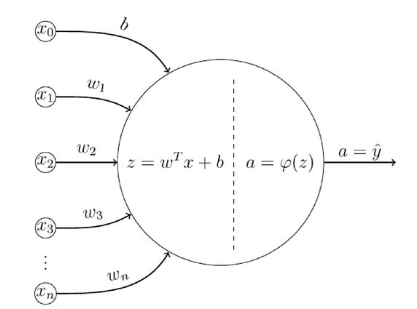
\includegraphics[width=0.46\linewidth]{Imagens/chap02/neuron_scheme.png}
    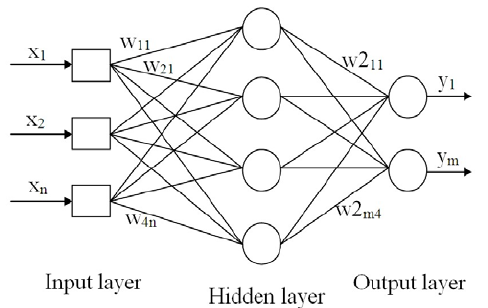
\includegraphics[width=0.46\linewidth]{Imagens/chap02/mlp_scheme.png}
    \caption{Esquema de neurônio (esquerda) e rede neural MLP (direita) \cite{minsky1969perceptrons}.}
    \label{fig:mlp_scheme}
\end{figure}

\subsubsection{Erros de estimação}
O treinamento da rede consiste, então, na minimização do erro entre $\hat{Y}$ e $Y$, que pode ser:
\begin{enumerate}
    \item Erro Absoluto Médio (MAE):
    \begin{equation}
        J_{MAE} = \frac{1}{m} \sum_{i=1}^m |y^{(i)} - \hat{y}^{(i)}|
    \end{equation}
    \item Erro Quadrático Médio (MSE):
    \begin{equation}
        J_{MSE} = \frac{1}{m} \sum_{i=1}^m (y^{(i)} - \hat{y}^{(i)})^2
    \end{equation}
    \item Entropia Cruzada: 
    \begin{equation}
        J_{CE} = -\frac{1}{m}[y^{(i)}\log(\hat{y}^{(i)}) + (1-y^{(i)})\log(1-\hat{y}^{(i)})]
    \end{equation}
\end{enumerate}

\subsubsection{\textit{Backpropagation}}
Este erro é utilizado para ajustar o vetor de pesos $\mathbf{w}$ e o viés $b$ da camada de saída através de otimizadores clássicos, e das demais camadas da rede neural através do algoritmo de \textit{backpropagation} \cite{hecht1992theory}, o cerne das redes neurais, que utiliza o ajuste de um neurônio para ajustar os neurônios conectados ao seus dendritos (entrada) conforme as equaçãões \ref{eq:backprop_start}-\ref{eq:backprop_end}:

\begin{align}
    \frac{\partial J}{\partial y_i} &= \frac{\partial J}{\partial o}\frac{\partial w}{\partial y_i} \label{eq:backprop_start}  \\
    y_i &= \phi(z) \\
    z &= \mathbf{w}^T\mathbf{x} + b \\
    \frac{\partial o}{\partial y_i} &= \frac{\partial o}{\partial z}\frac{\partial z}{\partial y_i}  = \frac{\partial o}{\partial z}w_i \label{eq:backprop_end}
\end{align}

onde $ \frac{\partial o}{\partial z}$ depende da função de ativação $\phi(z)$, $\frac{\partial J}{\partial o}$ é o ajuste conhecido do neurônio $o$, e $\frac{\partial J}{\partial y_i}$ é o ajuste estimado do neurônio $y_i$ conectado ao neurônio $o$ pelo peso $w_i$, como ilustrado na figura \ref{fig:backprop}.

\begin{figure}[hbt!]
    \centering
    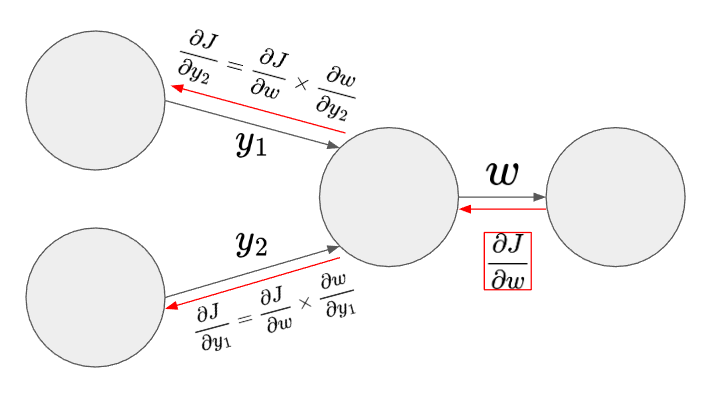
\includegraphics[width=0.8\linewidth]{Imagens/chap02/backprop.png}
    \caption{Ilustração do algoritmo de backpropagation. Fonte: o autor.}
    \label{fig:backprop}
\end{figure}

\subsubsection{Redes Neurais Convolucionais (CNN)}
As redes neurais convolucionais (CNN) são redes análogas às redes tradicionais como o MLP, no sentido de possuir um conjunto de neurônios que se otimizam a fim de aprender uma determinada tarefa. A diferença notável das redes convolucionais é a sua aplicação: para problemas que envolvem dados multidimensionais (tensores), como imagens, onde regiões próximas contém informações semelhantes, é recomendado o uso de CNNs. Isso porque ela permite a extração das características dessas imagens, que então alimentam uma rede MLP tradicional \cite{o2015introduction}, como ilustrado na figura \ref{fig:cnn_scheme}.

\begin{figure}[hbt!]
    \centering
    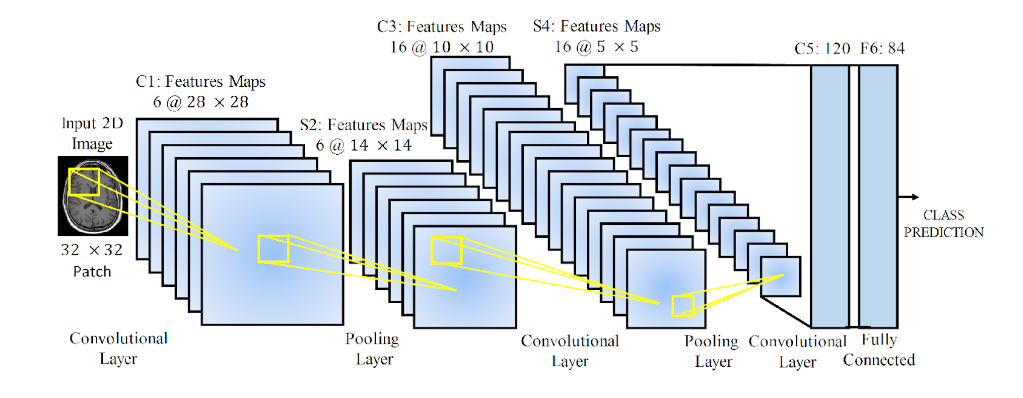
\includegraphics[width=0.8\linewidth]{Imagens/chap02/cnn_scheme.png}
    \caption{Esquema de uma CNN usada para análise de imagens de tomografia \cite{anwar2018medical}.}
    \label{fig:cnn_scheme}
\end{figure}

No caso das CNNs, em vez de valores únicos de pesos, cada conexão entre neurônios recebe uma matriz de pesos, chamados de filtros. Esses filtros então realizam uma operação de convolução com os dados recebidos (como ilustrado na figura \ref{fig:conv_scheme}), daí o nome da rede.

\begin{figure}[hbt!]
    \centering
    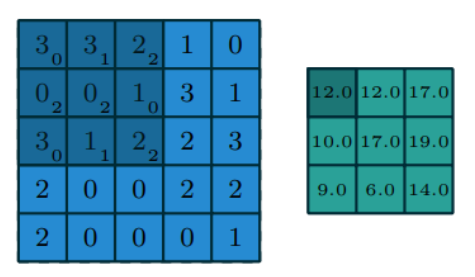
\includegraphics[width=0.5\linewidth]{Imagens/chap02/conv_scheme.png}
    \caption{Convolução entre o filtro (azule escuro) e os dados (azul claro). O resultado da convolução é a saída do neurônio (verde) \cite{odena2016deconvolution}.}
    \label{fig:conv_scheme}
\end{figure}

\subsubsection{Redes Neurais Recorrentes (RNN)}
As redes neurais recorrentes se destacam na solução de problemas que envolvem a identificação e modelagem de sistemas dinâmicos, utilizando dados de séries temporais. Por se tratar de dados que possuem algum interação estatística e temporal, a arquitetura das RNNs consiste numa cadeia de neurônios chamados células, que possuem um determinado estado oculto , que é definido como \cite{yu2019review}:
\begin{equation}
    y_t = h_t = \sigma(W_h h_{t-1}+W_xx_t+b)
\end{equation}

onde $h$ é o estado da célula, que depende do estado passado $h(t-1)$ pertencente a célula anterior, da entrada atual $x(t)$. $W_h$, $W_x$ são pesos e $b$ é um viés, todos os quais são parâmetros ajustados no treinamento.  A figura \ref{fig:rnn_cell} contém um esquema de uma célula de uma RNN.

\begin{figure}[hbt!]
    \centering
    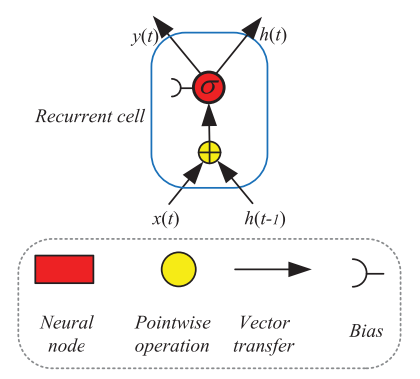
\includegraphics[width=0.5\linewidth]{Imagens/chap02/rnn_cell.png}
    \caption{Esquema de célula $\sigma$ recorrente padrão \cite{yu2019review}.}
    \label{fig:rnn_cell}
\end{figure}

Com o objetivo de lidar com problemas onde os dados das séries temporais possuem dependências estatísticas também a longo prazo, \cite{hochreiter1997long} propuseram a célula LSTM, que melhoraram a capacidade de memória da célula $sigma$ supracitada intoduzindo um "portão" dentro da célula. Este portão decide se a informação da entrada $x(t)$ vai ser jogada fora. O funcionamento da célula LSTM com portão de esquecimento ilustrada na figura \ref{fig:lstm_cell} é expresso como:
\begin{align}
    f_t &= \sigma(W_{fh}h_{t-1} + W_{fx}x_t + b_f) \\
    i_t &= \sigma(W_{ih}h_{t-1}+W_{ix}x_t+b_i) \\
    \Tilde{c}_t &= \tanh(W_{\Tilde{c}h}h_{t-1}+W_{\Tilde{c}x}x_t + b_{\Tilde{c}}) \\
    c_t &= f_t \cdot c_{t-1} + i_t \cdot \Tilde{c}_t \\   
    o_t &= \sigma(W_{oh}h_{t-1}+W_{ox}x_t+b_i) \\
    h_t &= o_t \cdot \tanh(c_t)
\end{align}

\begin{figure}[hbt!]
    \centering
    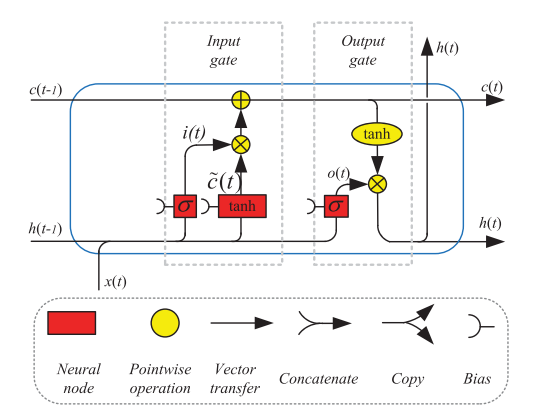
\includegraphics[width=0.6\linewidth]{Imagens/chap02/lstm_cell.png}
    \caption{Esquema de célula LSTM padrão \cite{yu2019review}.}
    \label{fig:lstm_cell}
\end{figure}

\newpage
\section{Controle MPC}
O Controle por Modelo Preditivo (MPC) é um método de controle eficiente e aplicado em diversos processos industriais. Ele consiste de três elementos básicos \cite{han2013nonlinear}:
\begin{enumerate}
    \item Modelo: Realiza a predição da evolução do sistema controlado, a partir da identificação da dinâmica do seu comportamento. Como o sistema modelado é não linear, o MPC desenvolvido é denominado NMPC. Pela complexidade da identificação desse sistema, surge a necessidade da utilização de redes neurais LSTM como a utilizada neste trabalho.
    \item Trajetória de referência: O comportamento alvo desjeado para as saídas do sistema, no caso a largura e altura do cordão.
    \item Otimizador: Estima o controle ótimo que minimiza uma determinada função custo estabelecida. Essa função geralmente possui duas parcelas: o erro de rastreamento e a regularização do sinal de controle.
\end{enumerate}

O comportamento preditivo do MPC permite, portanto, a previsão das saídas do sistema num determinado horizonte de tempo, possibilitando que ele não só rastreie uma determinada trajetória desejada como também minimize a função custo estabelecida. Ele é capaz de integrar controle ótimo, controle de processos, controle multivariável e referências futuras, simultâneamente \cite{han2013nonlinear}. A figura \ref{fig:mpc_scheme} ilustra a malha fechada de controle via NMPC.

\begin{figure}[hbt!]
    \centering
    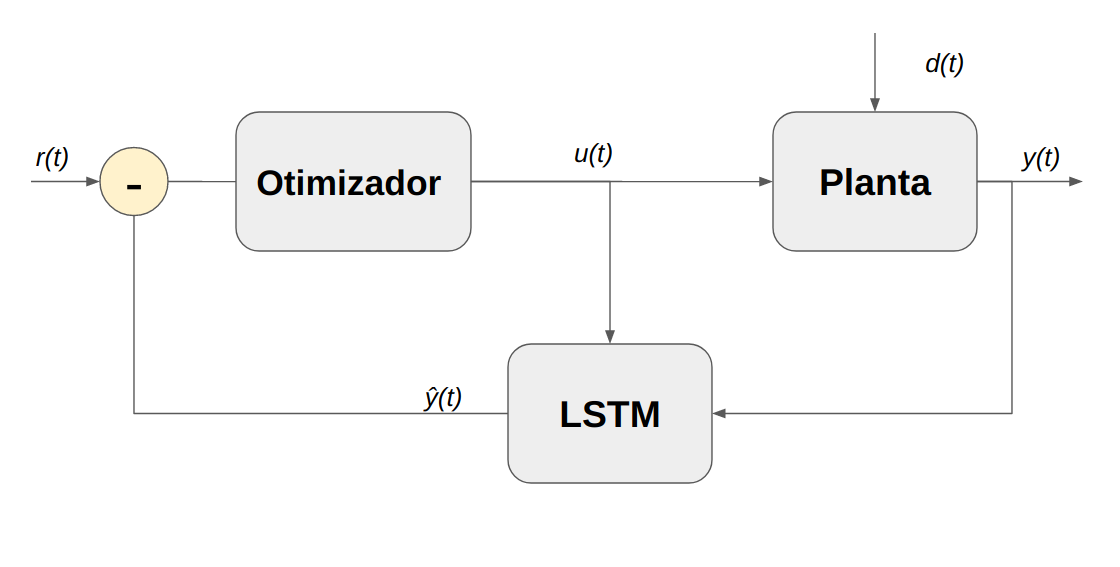
\includegraphics[width=0.7\linewidth]{Imagens/chap02/mpc_scheme.png}
    \caption{Esquema de malha fechada de controle via NMPC.}
    \label{fig:mpc_scheme}
\end{figure}

\subsection{Otimizador}
A otimização do controle NPMC em questão consiste na minimização de dois erros, o de rastreamento e de regularização, como no exemplo formulado abaixo:
\begin{align}
    \min_{U(t)} J(t) = \min_{U(t)} a \sum_{k=0}^{N-1}(r(t+k)&-y(t+k))^2 + b \sum_{k=0}^{M-1}u(t+k)^2 \\
    \text{sujeito a} \;\;\;\;& \\
    u_{min} \leq &u(t) \leq u_{max} \\
    y_{min} \leq &y(t) \leq y_{max}
\end{align}
onde $a$ e $b$ são pesos, $N$ o horizonte de predição da saída, $M$ o horizonte de predição de controle e $U(t)=[u(t), u(t+1), ..., u(t+M-1)]$ é o controle ótimo estimado. No instante $t$, calcula-se o controle $U(t)$ e utiliza como controle o primeiro ponto ($u^*(t) = U(t)$). Na seção \ref{sec:mpc_imp} será detalhada a otimização implementada neste trabalho.